\definecolor{Sail}{rgb}{0.643,0.819,0.976}
%%%%%%%%%%%%%%%%%%%%%%%%%%%%%%%%%%%%%%%%%%%%%%%%%%%%%%%%%%%%%%%%%%%%%%%%%%%%%%%%%%%%%%%%%%%%%%%%%%%%%%%%%%%%%%%%%%%%%%%%
\section{Principio de medición para sensores de ultrasonido}\label{ap:principioDeMedicionUltrasonido}

La velocidad y dirección del viento se determinan midiendo el tiempo que tardan los pulsos ultrasónicos en recorrer la distancia desde el transductor que genera el pulso hasta el transductor receptor. El instrumento utiliza dos pares de transductores orientados a lo largo de dos ejes ortogonales. Detectar la velocidad del viento a lo largo de dos ejes permite determinar no solo la intensidad sino también la dirección del viento.

El instrumento mide el tiempo de viaje del pulso ultrasónico entre los dos transductores de la misma pareja en ambas direcciones, como se muestra en la figura \ref{fig:trasductoresUltra}. Los tiempos de viaje en las dos direcciones opuestas se definen como $t_{A}$ (tiempo en dirección hacia adelante) y $t_{R}$ (tiempo en dirección inversa). Si la velocidad del viento es cero, los valores de $t_{A}$ y $t_{R}$ son iguales. En presencia de viento, uno de los dos valores de tiempo es mayor que el otro y la comparación entre los dos valores de tiempo permite determinar la dirección y la intensidad del viento.

\begin{figure}[H]
  \centering
  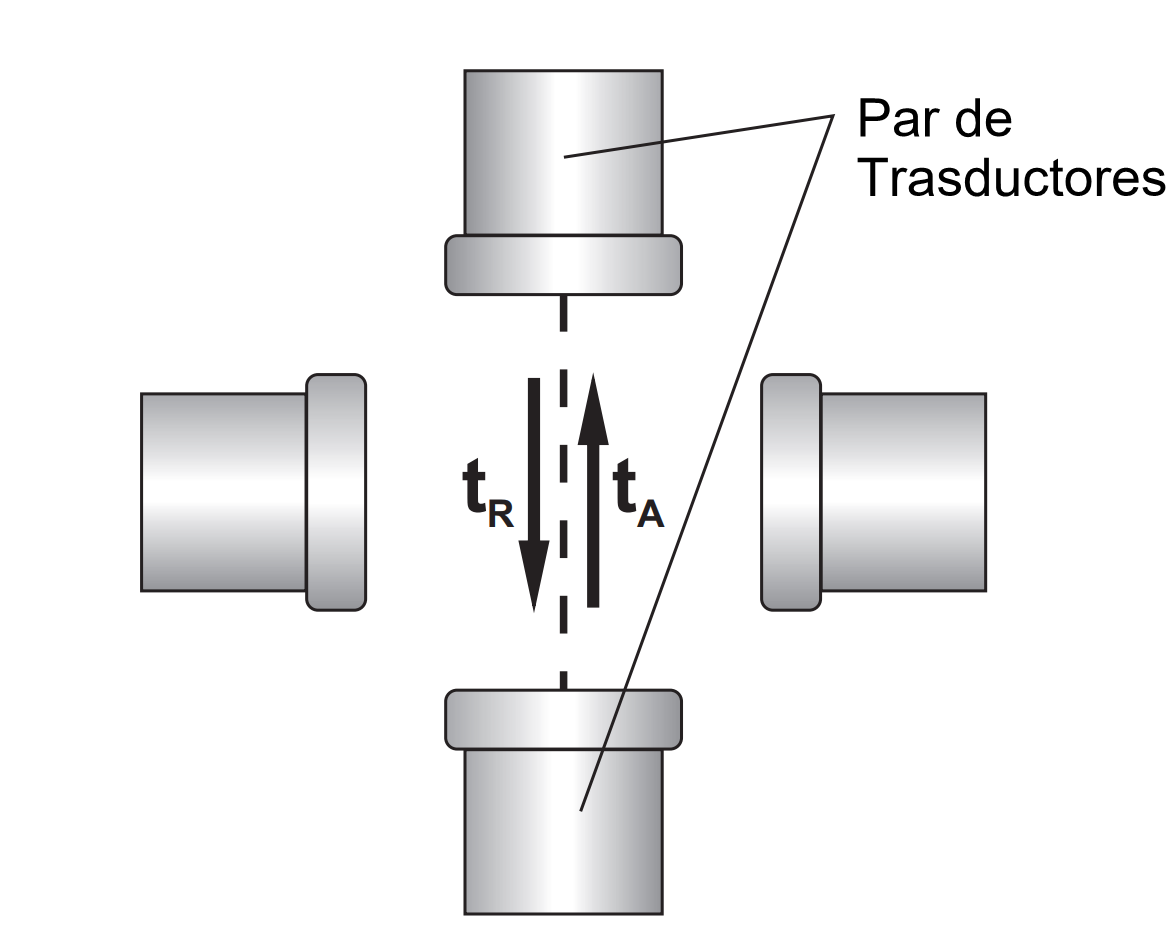
\includegraphics[width=0.4\textwidth]{Figuras/apendiceA/trasductoresUltra.png}
  \caption{Esquema de los transductores y el tiempo de viaje de un pulso ultrasónico. \cite{DeltaOHM_HD51.3D_manual}}
  \label{fig:trasductoresUltra}
\end{figure}

El tiempo de viaje del pulso de ultrasonido esta dado por las ecuaciones \ref{eq:t_A} y \ref{eq:t_R}
\begin{equation}
  t_{A} = \frac{D}{C + Vw}
  \centering
  \label{eq:t_A}
\end{equation}

\begin{equation}
  \centering
  t_{R} = \frac{D}{C - Vw}
  \label{eq:t_R}
\end{equation}

donde se define:
\begin{itemize}
  \item D: Distancia entre los dos transductores del mismo par.
  \item C: Velocidad del sonido.
  \item $V_{w}$: Componente de la velocidad del viento a lo largo del eje de medición.
\end{itemize}

Realizando la medición de los dos tiempos de viaje en los ejes cartesianos $\mathbf{U}$ y $\mathbf{V}$ podemos determinar el vector velocidad de viento como 


\begin{equation}
  \centering
  V_{w_{i}} = \frac{D}{2}\left(\frac{1}{t_{a_{i}}}-\frac{1}{t_{R_{i}}}\right)\text{,  } i= u,v
  \label{eq:velViento}
\end{equation}

El eje $\mathbf{U}$ es un eje que va de oeste a este, mientras que el eje $\mathbf{V}$ es un eje que va de sur a norte. Medir el tiempo de viaje en ambas direcciones permite cancelar la dependencia de la velocidad de transmisión de los ultrasonidos en el aire de las condiciones ambientales de temperatura, humedad y presión barométrica.



%%%%%%%%%%%%%%%%%%%%%%%%%%%%%%%%%%%%%%%%%%%%%%%%%%%%%%%%%%%%%%%%%%%%%%%%%%%%%%%%%%%%%%%%%%%%%%%%%%%%%%%%%%%%%%%%%%%%%%%%
\section{Especificaciones técnicas y hojas de datos}\label{EspecificacionesTecDataSheet}
\begin{table}[H]
\centering
\fontsize{10}{8}\selectfont
\begin{tblr}{
  row{1} = {Sail},
  row{6} = {Sail},
  row{11} = {Sail},
  row{16} = {Sail},
  column{2} = {c},
  cell{1}{1} = {c=2}{},
  cell{6}{1} = {c=2}{},
  cell{11}{1} = {c=2}{},
  cell{16}{1} = {c=2}{},
  hlines,
  vlines,
}
\textbf{Velocidad de viento}     &                                                                                           \\
Sensor                           & Ultrasonido                                                                               \\
Rango de Medición                & $\SI{0}{\meter\per\second}$ a $\SI{75}{\meter\per\second}$                                \\
Resolución                       & $\SI{0.1}{\meter\per\second}$                                                             \\                                 
Precisión                        & {$ \pm \SI{0.2}{\meter\per\second}$ o $2\%$ de la medición hasta $\SI{60}{\meter\per\second}$ \\ $3\%$ de la medición para mayor que $\SI{60}{\meter\per\second}$~}\\
\textbf{Dirección del viento}    &                                                                                           \\
Sensor                           & Ultrasonido                                                                               \\
Rango de Medición                & $\SI{0}{\degree}$ a $\SI{359.9}{\degree}$                                                \\
Resolución                       & $\SI{0.1}{\degree}$                                                                       \\
Precisión                        & $\pm \SI{2}{\degree} $ RMSE (velocidad del viento  $\SI{2}{\meter\per\second}$)           \\
\textbf{Fuente de alimentación}  &                                                                                           \\
Fuente de alimentación del calentador           & $\SI{24}{\volt}$ Vdc $\pm 10\%$\\
Consumo de energía del calentador               & $\SI{30}{\watt}$       \\
{Fuente de alimentación del\\ instrumento (sin calentador)}          & $\SI{12}{\volt}$ a $\SI{30}{\volt}$ Vdc\\
{Consumo de energía del\\ instrumento (sin calentador)}              & $\SI{60}{\milli\ampere}$ @ $\SI{24}{\volt}$ Vdc\\
\textbf{Otras especificaciones }    &                                                                                           \\
Salida Serial                       & RS232 aislado y  RS485                                                                      \\
Protocolo de comunicación           & NMEA, MODBUS-RTU, ACII propietario                                                               \\
Intervalo de medición               & Configurable de $\SI{250}{\milli\second}$ a $\SI{1}{\second}$\\
Intervalo de velocidad promedio     & Configurable de $\SI{1}{\second}$ a $\SI{10}{\minute}$\\
Conexión eléctrica                  & 19-pole M23 conector Macho\\
Temperatura de operación            & $\SI{-40}{\degreeCelsius}$ a $+\SI{70}{\degreeCelsius}$\\
Grado de protección                 &  IP66                                                                                         \\                                                                                 
\end{tblr}
\caption{Especificaciones de sensor de viento, marca Delta Ohm, modelo HD51.3.}
\label{tab:especTecniDelta}
\end{table}

\section{Sección 2}
